\documentclass[nobib]{tufte-handout}

\title{Lecture 8: Hamilton cycles, matchings, independent sets $\cdot$ 1MA020}

\author[Vilhelm Agdur]{Vilhelm Agdur\thanks{\href{mailto:vilhelm.agdur@math.uu.se}{\nolinkurl{vilhelm.agdur@math.uu.se}}}}

\date{15 November 2023}


%\geometry{showframe} % display margins for debugging page layout

\usepackage{graphicx} % allow embedded images
  \setkeys{Gin}{width=\linewidth,totalheight=\textheight,keepaspectratio}
  \graphicspath{{graphics/}} % set of paths to search for images
\usepackage{amsmath}  % extended mathematics
\usepackage{booktabs} % book-quality tables
\usepackage{units}    % non-stacked fractions and better unit spacing
\usepackage{multicol} % multiple column layout facilities
\usepackage{lipsum}   % filler text
\usepackage{fancyvrb} % extended verbatim environments
  \fvset{fontsize=\normalsize}% default font size for fancy-verbatim environments

\usepackage{color,soul} % Highlights for text

% Standardize command font styles and environments
\newcommand{\doccmd}[1]{\texttt{\textbackslash#1}}% command name -- adds backslash automatically
\newcommand{\docopt}[1]{\ensuremath{\langle}\textrm{\textit{#1}}\ensuremath{\rangle}}% optional command argument
\newcommand{\docarg}[1]{\textrm{\textit{#1}}}% (required) command argument
\newcommand{\docenv}[1]{\textsf{#1}}% environment name
\newcommand{\docpkg}[1]{\texttt{#1}}% package name
\newcommand{\doccls}[1]{\texttt{#1}}% document class name
\newcommand{\docclsopt}[1]{\texttt{#1}}% document class option name
\newenvironment{docspec}{\begin{quote}\noindent}{\end{quote}}% command specification environment

\include{mathcommands.extratex}

\begin{document}

\maketitle% this prints the handout title, author, and date

\begin{abstract}
\noindent
We begin by continuing to pursue consequences of the Ford-Fulkerson theorem, proving König's theorem.
\end{abstract}

\section{König's theorem}

In our last lecture, we proved the Ford-Fulkerson theorem relating minimum cuts and maximal flows, and used it to prove the Hall marriage theorem on matchings in bipartite graphs. We begin this lecture by proving another result we can derive from Ford-Fulkerson, namely König's theorem about vertex covers of bipartite graphs.

\begin{definition}
    Let $G$ be a finite simple graph. A \emph{vertex cover} of $G$ is a subset $S\subseteq V$ such that every edge has an endpoint in $S$. The \emph{covering number} of $G$, denoted $\beta(G)$, is the minimum size of any vertex cover of $G$.
\end{definition}

\begin{example}
    A star graph has covering number $1$, while a complete graph on $n$ vertices has covering number $n-1$. A cycle graph on $2n$ vertices has covering number $n$.
\end{example}

\begin{theorem}[König's theorem]
    Let $G$ be a bipartite graph. Then the maximum cardinality of a matching on $G$ equals $\beta(G)$, the minimum cardinality of a vertex cover of $G$.

    \begin{proof}
        Let $M$ be a maximal matching in $G$, and like in the proof of the marriage theorem, construct a flow network $G'$ from $G$. As we saw in the proof of that theorem, this matching $M$ corresponds to a maximal flow in $G'$ of value $\abs{M}$. By Ford-Fulkerson, this means there is a minimum cut $S, T$ on $G'$ of capacity $\abs{M}$.

        \begin{figure}
            \centering
            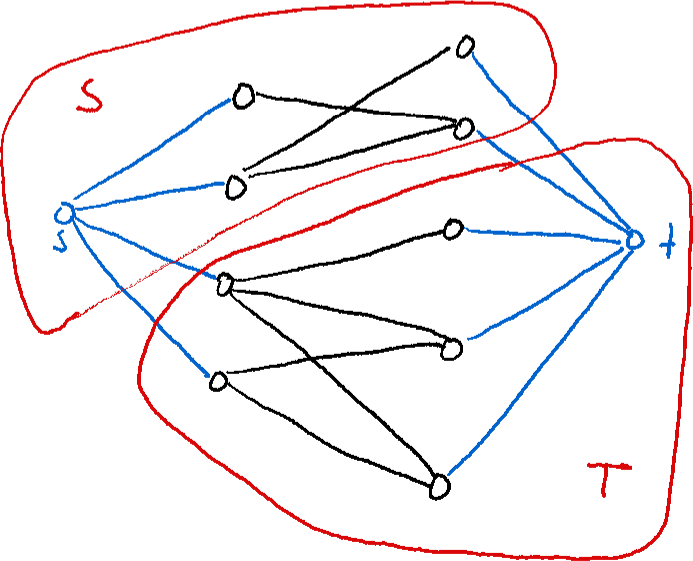
\includegraphics[width=0.5\textwidth]{graphics/L7_flows/bipartite_s_t_cut.png}
            \caption[][0cm]{A non-trivial minimal s-t-cut in a flow network created from a bipartite graph.}
            \label{fig:minimal_s_t_cut}
        \end{figure}

        Now, given this cut, let us construct a vertex cover. In particular, we let
        $$C = (A \cap T) \cup (B \cap S).$$
        That this $C$ is a vertex cover of $G$ is precisely the statement that there is no edge $a \to b$ with $a \in A \cap S$ and $b \in B \cap T$. This, however, is something we already saw is true for all minimum cuts in the previous proof -- because if there were such an edge, it would contribute $\infty$ to the capacity of the cut. So $C$ is indeed a vertex cover, and it is easy to convince oneself, looking at Figure \ref{fig:minimal_s_t_cut}, that $\abs{C} = c(S,T) = \abs{f} = \abs{M}$. So what we have seen is that the size of a maximal matching upper bounds the minimum vertex cover size, that is, $\beta(G) \leq \abs{M}$. 
        
        The other direction of the inequality in fact holds for all graphs, not just bipartite graphs -- every edge of a matching has to be covered by a vertex in the cover, and no vertex can cover more than one edge of the matching at a time. So any vertex cover has to have at least as many vertices in it as a maximal matching has edges.
    \end{proof}
\end{theorem}

\section{Hamilton cycles}

We studied, at the very beginning of the course, the notion of Eulerian circuits. The twin notion of Hamilton cycles appeared in our exercise session, but less us quickly repeat what we said about those.

\begin{definition}
    Let $G = (V,E)$ be a finite simple graph. A \emph{Hamilton cycle} in $G$ is a cycle that visits every vertex of $G$.\sidenote[][]{Recall that a \emph{cycle} by definition is a walk that starts and ends at the same vertex, and does not reuse any vertices other than the one it started with.} If $G$ admits a Hamilton cycle, we call it \emph{Hamiltonian}.
\end{definition}

Unlike for Eulerianity, there is no simple condition to determine whether a graph is Hamiltonian. In fact, computing whether a graph is Hamiltonian is an NP-Complete problem.

\begin{remark}
    Given a Hamiltonian cycle $C$ in $G$, we can easily construct a perfect matching of $G$ by just picking every second edge in the cycle. We can of course not in general turn a perfect matching into a Hamilton cycle, so Hamiltonicity is a stronger condition than having a perfect matching.
\end{remark}

That Hamiltonicity is an NP-Complete problem means we probably will never have any necessary and sufficient conditions for it. However, we can still prove results of the form ``if condition so-and-so holds, $G$ is Hamiltonian''. Let us prove the most famous such result.\sidenote[][]{It is named after a different Dirac than the one of quantum mechanics fame.}

\begin{theorem}[Dirac's theorem]
    Let $G = (V,E)$ be a simple graph on $n \geq 3$ vertices, such that every vertex has degree at least $\frac{n}{2}$. Then $G$ is Hamiltonian.

    \begin{proof}
        Assume $G$ is a graph satisfying the conditions of the theorem. Let us begin by observing that this $G$ cannot be disconnected -- if it were, the vertices in the smallest component would have fewer than half of the other vertices to connect to, so they would have too low degree.

        \begin{marginfigure}
            \centering
            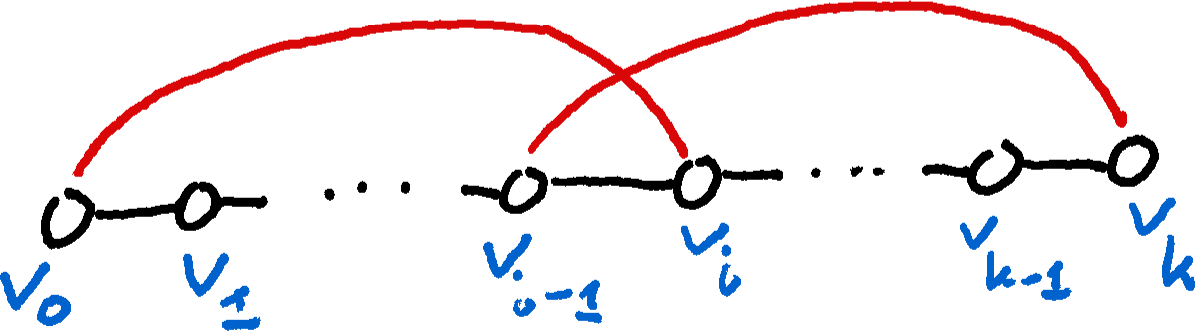
\includegraphics[width=1.0\textwidth]{graphics/L8_vx_covers_hamiltonicity_etc/diracs_thm_fig1.png}
            \caption{The path $P$ along with the configuration of two edges that must exist by the pigeonhole principle.}
            \label{fig:dirac_thm_fig1}
        \end{marginfigure}

        Now, consider a path $P$ of maximum length in $G$, say
        $$P = v_0\,e_1\,v_1\,\ldots\,v_{k-1}\,e_k\,v_k.$$
        Since this path is maximal, it contains all neighbours of $v_0$ and of $v_k$, since otherwise it could be extended. By our degree condition, there are (counting with multiplicity) at least $n$ such neighbours -- and so by essentially the pigeonhole principle, there must be an edge $e_i = \{v_{i-1},v_i\}$ on our path such that $v_i$ is a neighbour of $v_0$ and $v_{i-1}$ is a neighbour of $v_k$, as in Figure \ref{fig:dirac_thm_fig1}.

        Now we notice that this in fact lets us turn our path into a cycle -- we start at $v_0$, walk until $v_{i-1}$, then use the edge to $v_k$, walk backwards to $v_i$, and finally use the edge to $v_0$. This gives us a cycle $C$.

        \begin{marginfigure}
            \centering
            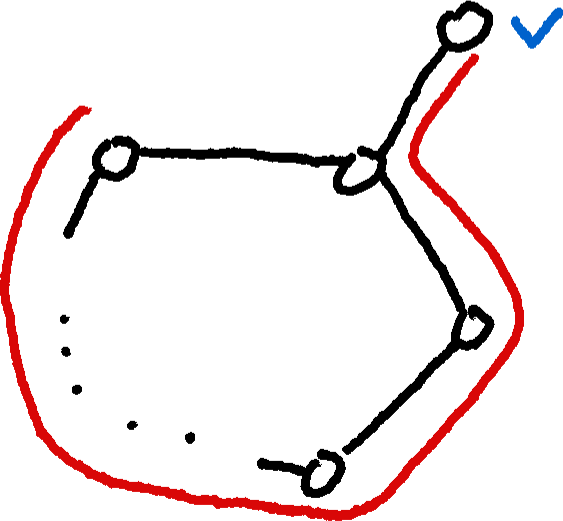
\includegraphics[width=0.6\textwidth]{graphics/L8_vx_covers_hamiltonicity_etc/diracs_thm_longer_path.png}
            \caption{A longer path than $P$ created from the cycle $C$, assuming it was not a Hamilton cycle.}
            \label{fig:diracs_thm_longer_path}
        \end{marginfigure}

        It remains to see that this $C$ is in fact a Hamilton cycle. So, suppose for contradiction that it is not, so that there is some vertex $v$ not on the cycle. Since $G$ is connected, we can in fact assume that this vertex is adjacent to some vertex of $C$. This, however, means we can create a longer path than $P$, by starting at $v$, walking onto $C$, and then following the cycle, as indicated in Figure \ref{fig:diracs_thm_longer_path}. However, we assumed $P$ was a maximal path, so we have a contradiction. So $C$ must be a Hamilton cycle.
    \end{proof}
\end{theorem}

\begin{figure}
    \centering
    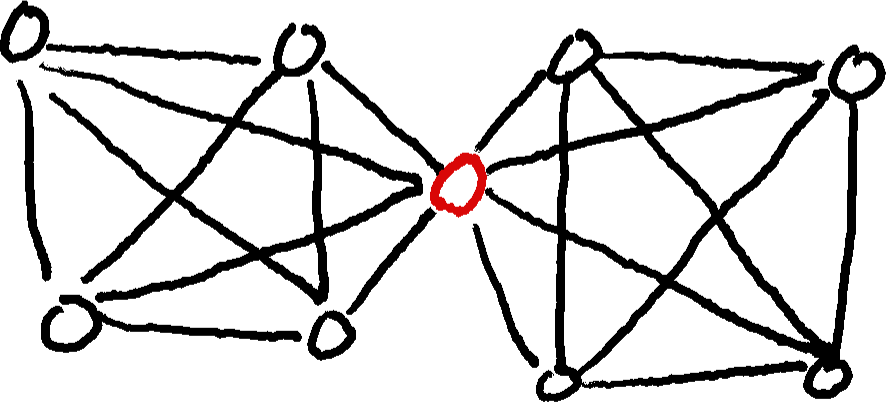
\includegraphics[width=0.65\textwidth]{graphics/L8_vx_covers_hamiltonicity_etc/diracs_theorem_counterexample.png}
    \caption[][0cm]{A graph used to show that the condition in Dirac's theorem is the best possible uniform lower bound.}
    \label{fig:dirac_counterexample}
  \end{figure}

\begin{remark}
    This result is in fact the best possible result with a uniform lower bound on the degrees of the vertices -- if we had picked any $k(n)$ less than $\frac{n}{2}$, there would be a counterexample. For example, consider the graph in Figure \ref{fig:dirac_counterexample}, where we have taken $k = \floor{\frac{n-1}{2}}$ and glued together two copies of $K_{k-1}$ by identifying two vertices. This graph has minimum degree $k$, but can of course not contain a Hamilton cycle since such a cycle would have to visit the glued-together vertex twice.
\end{remark}

Let us consider one particular example of a graph family that is Hamiltonian.

\begin{definition}
    The \emph{$d$-dimensional cube graph} has as its vertex set $\{0,1\}^d$, that is, the set of binary strings of length $d$. Two vertices are neighbours if the corresponding binary strings differ in only one position. The first few are illustrated in Figure \ref{fig:hypercubes}. 
\end{definition}

\begin{figure}
    \centering
    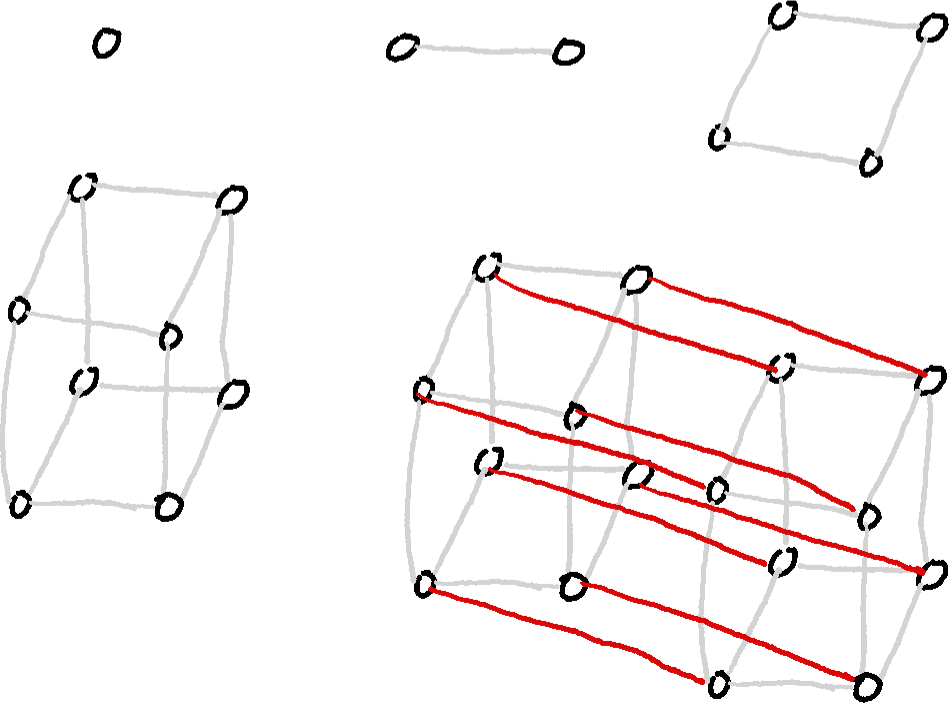
\includegraphics[width=0.65\textwidth]{graphics/L8_vx_covers_hamiltonicity_etc/binary_hypercubes.png}
    \caption[][0cm]{The $d$-dimensional cubes for $d = 0,1,2,4$. In the four-dimensional case we have highlighted some edges in red, to illustrate the inductive structure of the graph family.}
    \label{fig:hypercubes}
\end{figure}

\begin{theorem}\label{thm:hypercube_is_hamiltonian}
    The $d$-dimensional cube is Hamiltonian for all $d$.

    \begin{xca}
        Prove this.\qed
    \end{xca}
\end{theorem}

\begin{marginfigure}
    \centering
    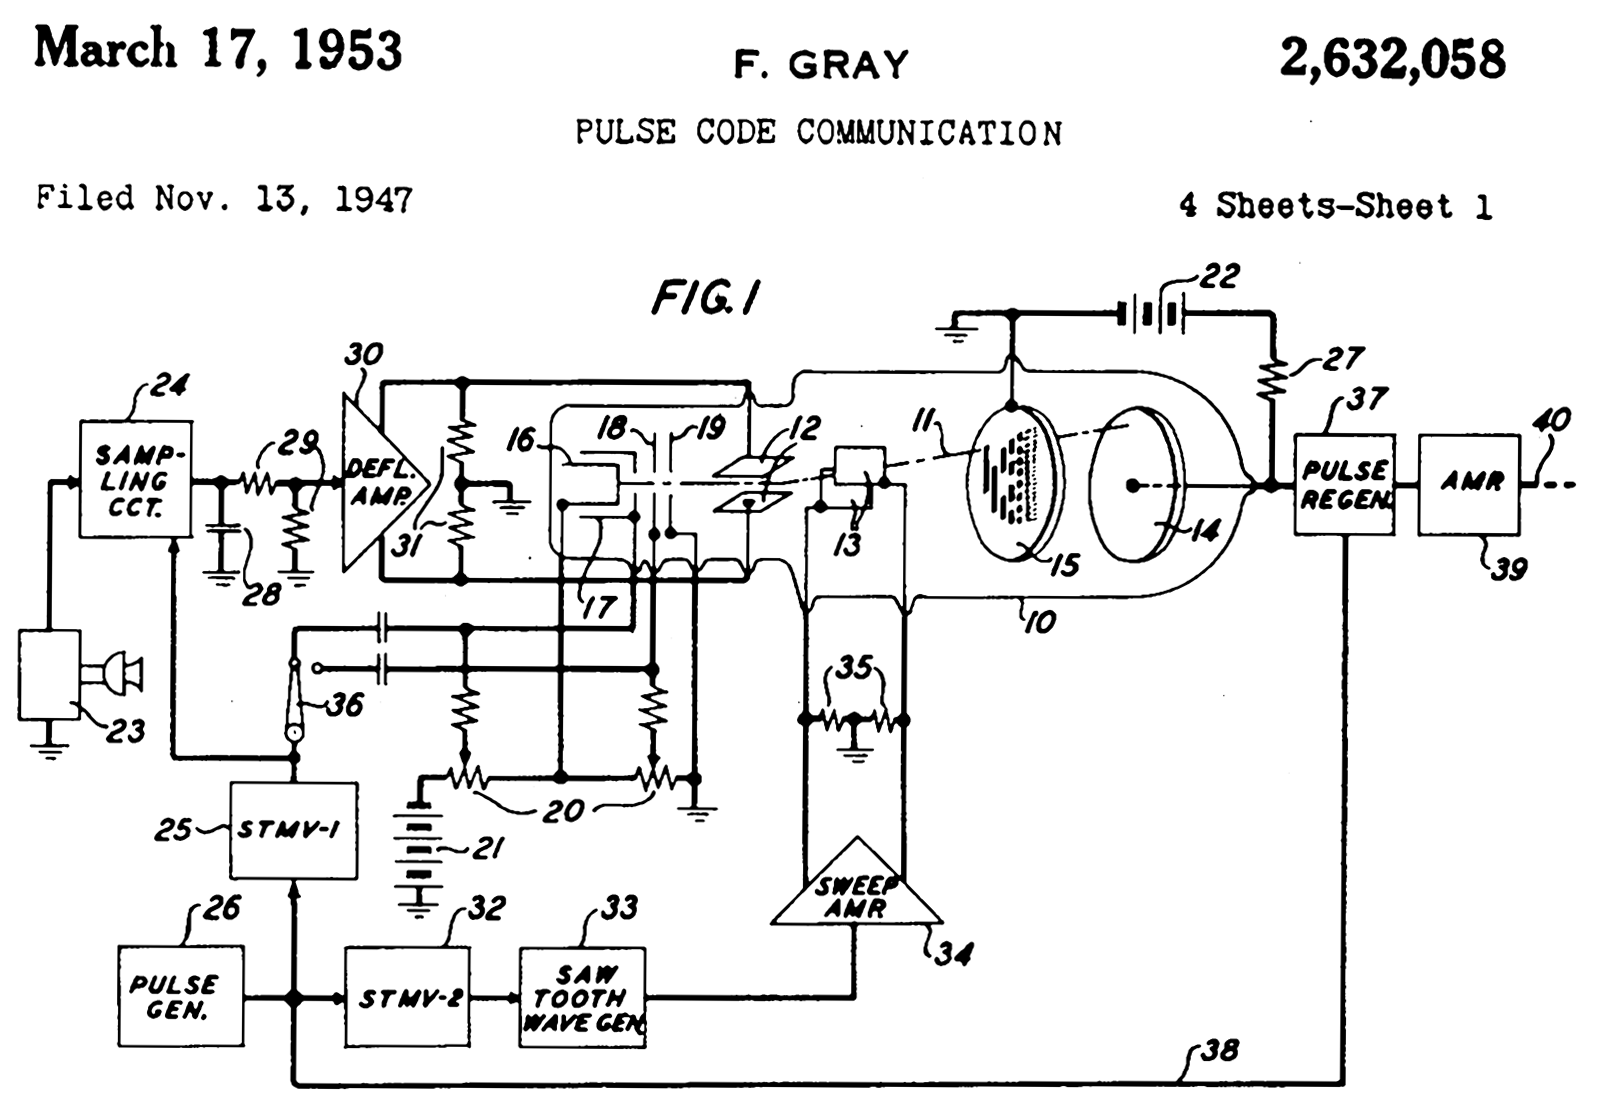
\includegraphics[width=1.0\textwidth]{graphics/L8_vx_covers_hamiltonicity_etc/gray_code_patent.png}
    \caption{The original patent for the device using a Gray code -- this supposedly happens in the thingy labelled by 15?}
    \label{fig:gray_code_patent}
\end{marginfigure}

\begin{remark}
    Notice that Theorem \ref{thm:hypercube_is_hamiltonian} gives us an ordering of the length-$d$ bit strings suh that going from one to the next always only requires us to change one of the bits. This ordering is known as the \emph{Gray code}, and it was originally invented to help in converting from analog to digital signals for colour television in the fifties.
\end{remark}

\section{Exercises}


%\bibliography{references}
%\bibliographystyle{plainnat}

\end{document}
